\subsection{System Arkitektur}

\begin{frame}{Hardware Komponenter (1)}
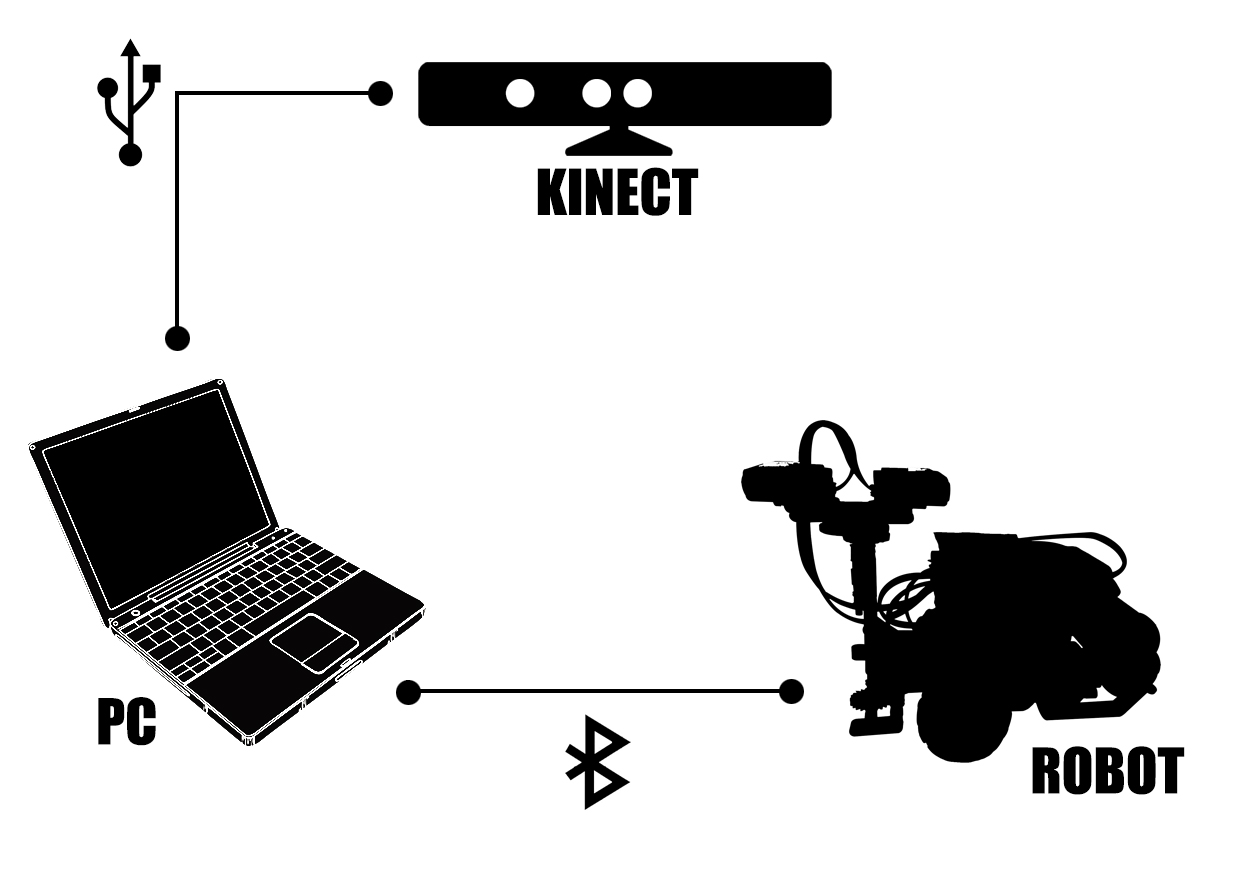
\includegraphics[width=\textwidth]{enheder}
\end{frame}

\begin{frame}{Hardware Komponenter (2)}
\begin{description}
\item[Kinect]{Billed-feed til lokalisering}
\item[NXT]{Navigation i/observation af verden}
\item[PC]{Beregning af:}
\begin{itemize}
\item{kort}
\item{robot lokation}
\item{rute}
\end{itemize}
\end{description}
\end{frame}

\begin{frame}{Hardware Komponenter (3)}
\begin{itemize}
\item{Proof of concept kontra anvendelighed;}
\begin{itemize}
\item{Mulighed for at isolere et enkelt problem}
\item{''Simulering'' af god lokationsberegning\\
samt højere regnekraft}
\end{itemize}
\item{Mulighed for udskiftning af komponent(er)}
\end{itemize}
\end{frame}

\subsection{NXT}

\begin{frame}{NXT Software (1)}
3 overordnede filer, med hver deres funktionalitet:
\begin{description}
\item[Sensor.nxc]{Observation af verden}
\item[Navigation.nxc]{Navigation i verden}
\item[Communication.nxc]{Kommunikation med PC}
\end{description}
\end{frame}

\begin{frame}{NXT Software (2)}
\begin{itemize}
\item{Selvstændig (embedded)}
\item{Ingen tunge beregninger}
\item{Gøre op for unøjagtiheder:}
\begin{itemize}
\item{Inkrementerende ''skridt'' ved navigering}
\item{Foretag 2 målinger ved lokation}
\end{itemize}
\end{itemize}
\end{frame}

\subsection{PC}

\begin{frame}{PC Software (1)}
Indsæt overordnet diagram (Yderste komponenter)
\end{frame}

\begin{frame}{PC Software (2)}
\begin{description}
\item[CommonLib]{DTOs, NXTPostMan, Interfaces}
\item[SystemInterface]{GUI og RobotInterface}
\item[Control]{Display, Location og Mapping}
\item[Services]{Robot, Route, Kinect, Tracking}
\item[Data]
\end{description}
\end{frame}

\begin{frame}{PC Software (3)}
\begin{itemize}
\item{Mange processer, samt tunge beregninger:}
\begin{itemize}
\item{Prioritering og samtidighed}
\end{itemize}
\item{Streng/meget arkitektur}
\begin{itemize}
\item{(Fordele/ulemper)}
\end{itemize}
\end{itemize}
\end{frame}

\subsection{Kommunikation}

\begin{frame}{Protokol}
\begin{description}
\item[Generelt]{$< BeskedType >< Indhold >$}
\item[Eksempel 1]{Robot anmoder om lokation\\
\texttt{0}}
\item[Eksempel 2]{PC sender lokation\\
\texttt{\textcolor{red}{52}-0213.5\textcolor{red}{00126.9}00187.4}}
\end{description}
\end{frame}

\begin{frame}{Flow}
Tilstandssekvensdiagram? Komponentdiagram? Vigtigt/spændende?
\end{frame}

\begin{frame}{Sidste tanker}
\end{frame}
